%==============================================================================
%  Nikah --- Islamic Nikah Matrimony Platform
%  CSE 400 : Software Development Project IV  |  Summer 2026
%  Final Project Report
%
%  Compile (any one):
%     pdflatex Final-SDP-Report.tex   (run 3x for TOC/LOF/LOT to settle)
%     latexmk -pdf Final-SDP-Report.tex
%
%  NOTE ON DOCUMENT CLASS
%  The cover supplied with this project was an IEEEtran/conference cover.
%  IEEEtran is a two-column, paper-oriented class with no \chapter support,
%  which is unsuitable for a long, chapter-based final report with wide
%  diagrams and tables. The cover page below is reproduced exactly (only the
%  heading is changed from LITERATURE REVIEW to PROJECT REPORT), but the body
%  uses the single-column "report" class so that chapters, the Table of
%  Contents, the List of Figures and the wide architecture/ER/DFD diagrams
%  render cleanly and professionally.
%==============================================================================
\documentclass[12pt,a4paper]{report}

%---------- Geometry & page setup ----------
\usepackage[a4paper,top=1.0in,bottom=1.0in,left=1.1in,right=1.1in,headheight=15pt]{geometry}
\usepackage{fancyhdr}
\usepackage{titlesec}
\titleformat{\chapter}[display]
  {\normalfont\huge\bfseries}{\chaptertitlename\ \thechapter}{10pt}{\Huge}
\titlespacing*{\chapter}{0pt}{-60pt}{20pt}

%---------- Encoding / fonts (pdflatex-safe, 7-bit ASCII diagrams) ----------
\usepackage[T1]{fontenc}
\usepackage[utf8]{inputenc}
\usepackage{lmodern}

%---------- Math, tables, graphics ----------
\usepackage{amsmath,amssymb}
\usepackage{graphicx}
\usepackage{booktabs}
\usepackage{array}
\usepackage{tabularx}
\usepackage{longtable}
\usepackage{multirow}
\usepackage{float}
\usepackage{caption}
\captionsetup{font=small,labelfont=bf}

%---------- Colour, lists, code, links ----------
\usepackage{xcolor}
\usepackage{enumitem}
\setlist[itemize]{leftmargin=*,topsep=2pt,itemsep=1pt}
\setlist[enumerate]{leftmargin=*,topsep=2pt,itemsep=1pt}
\usepackage{listings}
\usepackage{url}
\usepackage[hidelinks]{hyperref}

%---------- TikZ for diagrams ----------
\usepackage{tikz}
\usetikzlibrary{positioning,arrows.meta,shapes.geometric,shapes.misc,calc,fit,backgrounds}

%---------- Brand palette (emerald + gold, matching the app) ----------
\definecolor{emerald}{HTML}{047857}
\definecolor{emeraldlight}{HTML}{10B981}
\definecolor{gold}{HTML}{C99A2E}
\definecolor{slate}{HTML}{475569}
\definecolor{codebg}{HTML}{F6F8F7}

%---------- Listings styles (code + ASCII diagrams) ----------
\lstdefinelanguage{JavaScript}{
  morekeywords={const,let,var,function,return,if,else,for,await,async,new,try,catch,require,module,exports,true,false,null,typeof},
  morecomment=[l]{//},
  morestring=[b]',
  morestring=[b]"
}
\lstset{
  basicstyle=\ttfamily\footnotesize,
  backgroundcolor=\color{codebg},
  breaklines=true,
  frame=single,
  framerule=0.3pt,
  rulecolor=\color{slate!40},
  keywordstyle=\color{emerald}\bfseries,
  commentstyle=\color{slate}\itshape,
  stringstyle=\color{gold!80!black},
  showstringspaces=false,
  numbersep=6pt,
  xleftmargin=10pt
}
\lstdefinestyle{ascii}{
  language=,
  basicstyle=\ttfamily\scriptsize,
  frame=single,
  numbers=none,
  keywordstyle=,
  commentstyle=,
  stringstyle=,
  backgroundcolor=\color{codebg}
}

%---------- Headers / footers ----------
\pagestyle{fancy}
\fancyhf{}
\fancyhead[L]{\small\itshape Nikah --- Islamic Matrimony Platform}
\fancyhead[R]{\small CSE 400 \textbar{} SDP IV}
\fancyfoot[C]{\thepage}
\renewcommand{\headrulewidth}{0.4pt}
\fancypagestyle{plain}{%
  \fancyhf{}\fancyfoot[C]{\thepage}\renewcommand{\headrulewidth}{0pt}}

%---------- Reference / appendix names ----------
\renewcommand{\bibname}{References}
\renewcommand{\contentsname}{Table of Contents}

%---------- Helper: UI screenshot loader / placeholder ----------
\newcommand{\uifig}[3]{%
  \begin{figure}[H]
  \centering
  \IfFileExists{#3}{%
    \includegraphics[width=0.88\textwidth]{#3}%
  }{%
    \setlength{\fboxsep}{10pt}\setlength{\fboxrule}{0.4pt}%
    \fcolorbox{slate!40}{codebg}{%
      \begin{minipage}[c][5.2cm][c]{0.88\textwidth}\centering
        \itshape\small \detokenize{#3}
      \end{minipage}}%
  }%
  \caption{#1}\label{#2}
  \end{figure}}

%---------- Safe graphics: degrade to a placeholder box if a file is missing
\newcommand{\safegfx}[2]{%
  \IfFileExists{#2}{\includegraphics[#1]{#2}}{%
    \setlength{\fboxsep}{8pt}\setlength{\fboxrule}{0.4pt}%
    \fcolorbox{slate!40}{codebg}{%
      \begin{minipage}[c][4cm][c]{0.9\textwidth}\centering
        \itshape\small [image not found: \detokenize{#2}]
      \end{minipage}}}}

\begin{document}

%==============================================================================
%  COVER PAGE  (identical layout; heading = PROJECT REPORT)
%==============================================================================
\begin{titlepage}
\thispagestyle{empty}
\vspace*{0.4cm}
\noindent
\begin{minipage}{0.15\textwidth}
    \IfFileExists{bubtlogo.png}{%
        \includegraphics[width=\linewidth]{bubtlogo.png}%
    }{%
        \framebox[\linewidth]{\rule{0pt}{0.8\linewidth}\centering\small BUBT}%
    }
\end{minipage}%
\begin{minipage}{0.85\textwidth}
    \centering
    \large \textbf{Bangladesh University of Business and Technology}\\[1ex]
    \large Department of Computer Science and Engineering
\end{minipage}

\vspace{1.5cm}

\begin{center}
    \Large CSE 400 : Software Development Project IV
\end{center}

\vspace{1cm}

\begin{center}
    \Huge \textbf{PROJECT REPORT}
\end{center}

\vspace{1.5cm}

\noindent
\textbf{Semester:} \textcolor{blue!70!black}{Summer 2026}\\[1.5ex]
\textbf{Title:} Nikah --- Islamic Nikah Matrimony Platform\\[1.5ex]
\textbf{Submission Date:} \textcolor{blue!70!black}{August 2026}

\vspace{1.5cm}

\begin{center}
    \textbf{TEAM MEMBERS}\\[2ex]

    \renewcommand{\arraystretch}{1.3}
    \begin{tabular}{|c|c|c|}
        \hline
        \textbf{Full ID} & \textbf{Full Name} & \textbf{Intake/Section} \\
        \hline
        22235103137 & Md. Mahamudul Hasan & 51/11 \\
        \hline
        22235103251 & Sumya Soma & 51/11 \\
        \hline
        22235103411 & Salat Mahmud Chowdhury & 51/11 \\
        \hline
        22235103680 & Alfa Sany & 51/11 \\
        \hline
        22235103321 & Zinat Parvin & 51/11 \\
        \hline
    \end{tabular}
\end{center}

\vspace{2cm}

\begin{center}
    \textbf{SUPERVISED BY}\\[2ex]
    \textbf{Ahmed Shafkat}\\
    Assistant Professor, Department of CSE\\
    Bangladesh University of Business and Technology (BUBT)
\end{center}
\end{titlepage}

%==============================================================================
%  FRONT MATTER
%==============================================================================
\pagenumbering{roman}

%---------- Abstract ----------
\chapter*{Abstract}
\addcontentsline{toc}{chapter}{Abstract}
\noindent
\textbf{Nikah} is a full-stack, Islamic matrimony web platform designed for the
Bangladeshi Muslim community. It provides a private, secure and
religion-aligned environment in which individuals can build detailed
\emph{biodata} (matrimonial profile) records, search for compatible partners,
communicate through verifiable channels, and progress towards \emph{Nikah} ---
the Islamic marriage contract. The presentation tier is a single-page
application built with \textbf{React 18} and \textbf{Vite}, styled with
\textbf{Tailwind CSS} and the \textbf{shadcn/ui} component system (new-york
style, built on Radix UI), themed with a custom emerald-and-gold design token
set. The application tier is a \textbf{Node.js / Express 5} REST API, and the
data tier is \textbf{MongoDB Atlas} managed through the \textbf{Mongoose 9}
ODM across thirteen collections. Authentication is hybrid: regular members
authenticate through \textbf{Firebase} (email/password and Google) and exchange
their verified identity for a short-lived server JSON Web Token (JWT), while a
\textbf{dedicated administrator} authenticates against environment-configured
credentials issued by the server itself --- completely separate from Firebase.
Role-based access control (RBAC) distinguishes three tiers: regular user,
premium subscriber, and administrator. The platform delivers fifteen functional
modules including biodata management, filtered search, a compatibility matching
engine, contact-request workflow with payment gating, favourites, messaging,
notifications, profile-view tracking, recently-viewed history, premium
subscriptions, success stories, a reporting system, and a rich analytics-driven
admin dashboard. Uniquely for the market, several modules implement Islamic
principles directly: a \emph{deen}-weighted compatibility engine (with religion
as the largest scoring factor), a \emph{wali} (guardian) oversight workflow on
the contact-request path, NID/imam profile verification, halal-communication
message templates, a mahr preference field, and an Islamic guidance hub. The interface is bilingual (English / Bangla), fully
responsive, ships with a dark mode, and is deployed on free-tier cloud
infrastructure --- the API on Vercel, the front end on Netlify, and the database
on MongoDB Atlas.

\vspace{1em}
\noindent\textbf{Keywords:} Islamic matrimony, MERN stack, React, Express,
MongoDB, Firebase, JWT, role-based access control, shadcn/ui, responsive web
design, internationalization, Bangladesh.

%---------- Acknowledgment ----------
\chapter*{Acknowledgment}
\addcontentsline{toc}{chapter}{Acknowledgment}
\noindent
We express our sincere gratitude to our supervisor, \textbf{Mr.\ Ahmed Shafkat},
Assistant Professor, Department of Computer Science and Engineering, Bangladesh
University of Business and Technology (BUBT), for his continuous guidance,
valuable suggestions and encouragement throughout the development of this
project. We are also thankful to the faculty members of the Department of CSE
for their support and to the open-source community whose libraries and
documentation made this work possible. Finally, we thank our families for their
patience and encouragement during the entire Software Development Project IV
cycle.

%---------- Table of contents / list of figures / list of tables ----------
\tableofcontents
\cleardoublepage
\addcontentsline{toc}{chapter}{List of Figures}
\listoffigures
\cleardoublepage
\addcontentsline{toc}{chapter}{List of Tables}
\listoftables
\cleardoublepage

%==============================================================================
%  MAIN MATTER
%==============================================================================
\pagenumbering{arabic}

%==============================================================================
\chapter{Introduction}
%==============================================================================

\section{Problem Specification}
Marriage occupies a sacred position in Islam. The Prophet Muhammad (peace be
upon him) is reported to have said, \emph{``When a person marries, he has
fulfilled half of his religion''} (reported by al-Bayhaqi). Today the majority
of people turn to the internet when searching for a life partner, yet the
platforms that are widely available do not serve the Bangladeshi Muslim
community well.

Leading matrimony services such as \textbf{Shaadi.com} and \textbf{Muslima.com}
address a global audience and are not built around Islamic values; family
involvement, privacy in accordance with the principle of \emph{hijab}, and
religious compatibility are largely absent. Personal contact information is
frequently exposed without proper consent, creating genuine risks of harassment
and data misuse. Language is a further barrier: most Bangladeshi users prefer
Bangla, yet the dominant platforms operate in English. Pricing is prohibitive,
mobile optimization is poor despite mobile being the primary means of internet
access in Bangladesh, fake profiles are common, and there is no reliable way to
verify authenticity or to report suspicious activity.

These gaps motivated the construction of a platform that is modern, secure,
Islamically aligned and built specifically for Bangladeshi users --- the gap
that \textbf{Nikah} is designed to fill.

\section{Objectives}
The principal objectives of the project were:
\begin{enumerate}
  \item To build a complete matrimony platform with a React front end, a
        Node.js/Express back end and a MongoDB database.
  \item To design features that respect Islamic values --- privacy, family
        involvement and halal communication.
  \item To allow members to create and manage detailed biodata profiles with
        personal, family and partner-preference information.
  \item To provide rich search filters and a compatibility matching engine
        based on age, height, division and occupation.
  \item To secure the platform with JWT authentication, role-based access
        control and contact-information gating.
  \item To keep the architecture modular so that it can scale as the user base
        grows.
  \item To support both English and Bangla through internationalization.
  \item To deliver a professional administration dashboard with analytics, a
        premium subscription model, user-to-user messaging and a fully
        responsive, dark-mode-capable interface.
\end{enumerate}

\section{Scope}
The scope of the project encompasses the complete design, development and
cloud deployment of a web-based matrimony platform. In scope are: user
registration and authentication (including a separate, secure administrator
login); biodata lifecycle management; filtered search and a compatibility
matching engine; contact-request workflow with payment gating; favourites,
messaging and notifications; profile-view tracking and recently-viewed history;
premium subscriptions and success stories; a reporting system; and a
analytics-rich admin dashboard. Bilingual (English/Bangla) support, a dark
theme, responsive design and cloud deployment (Vercel, Netlify, MongoDB Atlas)
are also in scope.

Out of scope for this phase are native mobile applications, real-time
WebSocket-based chat, live payment processing (the Stripe integration runs in
demonstration mode), machine-learning-based recommendations, and identity
verification --- these are discussed under future work.

\section{Flow of the Project}
Development was organized into six phases:
\begin{description}[leftmargin=2.2em]
  \item[Phase 1 --- Planning \& Design (Weeks 1--2):] Requirements gathering,
        use-case modelling, ER design, architecture planning and UI wireframing.
  \item[Phase 2 --- Back-End Development (Weeks 3--5):] MongoDB schema design
        with Mongoose, Express server bootstrap, JWT authentication, the
        environment-based administrator login, and CRUD endpoints for every
        collection.
  \item[Phase 3 --- Front-End Development (Weeks 6--9):] React/Vite scaffold,
        React Router configuration, Tailwind and shadcn/ui theming, Axios-based
        API integration, and construction of all pages.
  \item[Phase 4 --- Feature Enhancement (Weeks 10--11):] Messaging,
        notifications, the compatibility matching engine, profile-view tracking,
        recently-viewed history and premium subscription handling.
  \item[Phase 5 --- Testing \& QA (Weeks 12--13):] API testing with Postman,
        UI testing, accessibility checks, bug fixing and the security
        hardening of administrator access.
  \item[Phase 6 --- Deployment \& Documentation (Weeks 14--15):] Deployment of
        the API to Vercel and the front end to Netlify, environment-variable
        configuration, report writing and presentation preparation.
\end{description}

\section{Organization of the Project Report}
The remainder of this report is organized into six chapters.
\textbf{Chapter~2} surveys existing systems and the supporting literature.
\textbf{Chapter~3} presents the system analysis and design --- the technology
stack, the development model, the system architecture, the use-case, context
and data-flow diagrams, the database schema, and the core algorithms.
\textbf{Chapter~4} describes the implementation of the front end and back end
and enumerates the functional modules. \textbf{Chapter~5} is a user manual
covering system requirements and interface walkthroughs. \textbf{Chapter~6}
concludes with a discussion of limitations and future work, followed by the
references and appendices.

%==============================================================================
\chapter{Background and Related Works}
%==============================================================================

\section{Existing System Analysis}
Before constructing Nikah, the team examined the platforms already available in
order to understand where the gaps lay. Table~\ref{tab:competitors} summarises
the strengths and weaknesses of the most relevant competitors.

\begin{table}[H]
\centering
\caption{Comparative analysis of existing matrimony platforms.}
\label{tab:competitors}
\small
\renewcommand{\arraystretch}{1.25}
\begin{tabularx}{\textwidth}{l X X}
\toprule
\textbf{Platform} & \textbf{Strengths} & \textbf{Weaknesses} \\
\midrule
Shaadi.com       & Large user base, global reach       & Not Islam-specific, expensive, English-only \\
Muslima.com      & Muslim audience, international       & Outdated interface, limited Bangla, costly  \\
Biyeta (BD)      & Largest Bangladeshi Muslim user base, Bangla, halal branding, mobile app & Fake-profile complaints, weak verification, no structured compatibility algorithm, no wali-in-the-loop, costly premium \\
BiyeKotha (BD)   & Bangla support, local focus          & Poor UI, limited features, not mobile-friendly \\
Muzz (Muzmatch)  & Muslim-focused, modern, app-based, optional chaperone & Casual-dating framing, heavy premium model, few free features, weak Bangla \\
Tinder / Bumble  & Modern interface, large user base    & Not for marriage, no Islamic alignment \\
\midrule
\textbf{Nikah (this work)} & \textbf{Islamic-by-design flow (wali oversight, deen-compatibility scoring, halal-communication templates, NID/imam verification), Bangla + English, freemium, admin analytics} & \textbf{New platform (smaller initial user base than incumbents)} \\
\bottomrule
\end{tabularx}
\end{table}

The recurring gaps identified were:
\begin{itemize}
  \item No single platform combines a modern interface, Islamic values and
        Bangla support.
  \item None incorporates a \emph{religious} (deen) dimension into its
        compatibility engine --- religion is at most a search filter, never a
        matching factor.
  \item None builds \emph{wali} (guardian) consent into the contact-request
        flow; at best an optional ``chaperone'' feature exists.
  \item Verification against fake profiles is weak or absent across the board.
  \item None offers a structured compatibility matching algorithm.
  \item Administrator dashboards with analytics are absent across the board.
  \item Role-based access with a premium tier is not implemented.
  \item Real-time-style messaging and notification systems are missing.
  \item Profile-view tracking and recently-viewed history are not provided.
\end{itemize}

Nikah addresses every one of these gaps: it unifies a modern shadcn/ui and
Tailwind interface with Islamic privacy controls, full Bangla support, a
\emph{deen-weighted} compatibility engine (with religion as the largest scoring
factor), built-in \emph{wali} oversight of contact requests, NID/imam profile
verification, halal-communication templates, an analytics dashboard, messaging,
notifications and a freemium subscription model.

\section{Supporting Literatures}
The work draws on several bodies of knowledge --- Islamic teachings on marriage,
modern web architecture patterns, authentication frameworks, and the specific
front-end and back-end technologies employed.

\paragraph{Islamic foundations.} Nikah is deliberately Islamic-by-design rather
than Islamic-by-filter: every distinctive module maps to a recognised Islamic
principle, so the platform is not merely a generic matrimony engine with a
green theme. Table~\ref{tab:islamic-mapping} summarises this mapping, which
constitutes the project's core value proposition.

\begin{table}[H]
\centering
\caption{Mapping of Nikah modules to Islamic principles.}
\label{tab:islamic-mapping}
\small
\renewcommand{\arraystretch}{1.25}
\begin{tabularx}{\textwidth}{l X}
\toprule
\textbf{Module} & \textbf{Islamic principle it implements} \\
\midrule
Deen-compatibility matching & The Prophet (peace be upon him) directed: ``A woman is married for four things --- her wealth, her lineage, her beauty and her religious commitment; so marry the religious one, you will prosper'' (Sahih al-Bukhari~5090). Religion is therefore weighted as the single largest factor ($35\%$) in the score. \\
Wali (guardian) oversight & A valid nikah requires the consent of the \emph{wali} (Qur'an~4:25). Each contact request to a wali-protected profile must be approved by the guardian via a single-use magic link before contact details are shared. \\
Contact gating (\emph{hijab}) & Personal contact information is hidden until a verified, paid or premium request --- preserving modesty and consent, never exposing details casually. \\
Halal communication & Initial contact is scaffolded by respectful, marriage-intent message templates; senders may CC the recipient's wali; and an etiquette reminder keeps interaction purposeful, discouraging casual mixing. \\
Mahr preference field & The \emph{mahr} is the wife's Qur'anic right (Qur'an~4:4). Surfacing it on the biodata sets expectations transparently before any commitment. \\
Profile verification (NID/imam) & Deception (\emph{ghish}) is prohibited in Islam. NID- or imam-endorsed verification combats fake profiles and builds trust. \\
Guidance hub & Educational content on choosing a spouse, istikhara, mahr, wali and marital rights is offered as \emph{sadaqah jariyah} (perpetual charity), adding value beyond matching. \\
\bottomrule
\end{tabularx}
\end{table}

Three further points reinforce this foundation. First, the hadith that
``when a person marries, he has completed half of his religion'' (al-Bayhaqi)
motivates the entire platform: a tool that helps Muslims complete that half
\emph{halal}ly is itself an act of worship. Second, the platform respects the
principle of \emph{hijab} by gating contact information, and captures both
parents' names so that families remain central. Third, wali oversight is
modelled as a real workflow rather than a label --- the guardian receives a
verifiable approval link and can approve or decline each suitor, mirroring the
protective role the guardian holds in Islamic marriage.

\paragraph{Architecture.} The system follows a classical three-tier pattern:
a React single-page presentation layer, an Express REST application layer with
modular routers, and a MongoDB data layer managed by Mongoose.

\paragraph{Authentication and authorization.} Members authenticate through
Firebase (email/password and Google OAuth) and exchange the verified identity
for a server-issued JWT with a seven-day expiry. The administrator authenticates
separately against environment-configured credentials. A three-tier RBAC scheme
(user, premium, admin) is enforced by Express middleware.

\paragraph{Front-end stack.} React 18 was chosen for its ecosystem; Vite
provides fast builds and hot-module replacement; Tailwind CSS with
\texttt{darkMode:'class'} and the shadcn/ui component system (built on Radix UI
primitives) deliver an accessible, consistent and themeable UI; TanStack React
Query manages server state with caching; and Framer Motion supplies animation.

\paragraph{Back-end stack.} Node.js and Express~5 form the server; Mongoose~9
provides the ODM layer; Stripe handles payments (in demonstration mode); and
\texttt{bcryptjs} and \texttt{jsonwebtoken} provide password hashing and token
signing/verification respectively.

\paragraph{Database and deployment.} MongoDB Atlas offers a free, cloud-hosted
tier with auto-scaling; thirteen collections were designed with indexes on
frequently queried fields. The API runs as serverless functions on Vercel and
the front end is served by Netlify with continuous deployment from Git.

\section{Problem Statement and Research Gap}
The specific problem this project solves can be stated as follows:
\emph{Bangladeshi Muslims lack a single, trustworthy online platform that
simultaneously (a) respects Islamic privacy and family involvement --- including
real \emph{wali} (guardian) consent in the contact flow, (b) matches on
religious compatibility (\emph{deen}) and not only on age, location or
appearance, (c) speaks their language, (d) matches compatibility systematically
rather than only by free-text search, (e) protects contact information behind
verified access, and (f) gives operators meaningful administrative oversight.}
Existing solutions each satisfy at most one or two of these requirements.
Nikah is the integrated response to that research gap: an Islamic marriage
process delivered as software, rather than a matrimony site that merely permits
Muslim users.

%==============================================================================
\chapter{System Analysis and Design}
%==============================================================================

\section{Technology and Tools}

\subsection{Front-End Stack}
\begin{table}[H]
\centering
\caption{Front-end technologies and their roles.}
\label{tab:frontend}
\small
\begin{tabularx}{\textwidth}{l l X}
\toprule
\textbf{Technology} & \textbf{Version} & \textbf{Role} \\
\midrule
React.js                 & 18.3.1   & UI framework \\
Vite                     & 7.2.4    & Build tool and dev server \\
React Router DOM         & 7.10.1   & Client-side routing \\
Tailwind CSS             & 3.4.17   & Utility-first styling \\
shadcn/ui (new-york)     & ---      & Component system (Radix UI based) \\
Radix UI primitives      & 16 pkgs  & Accessible headless components \\
TanStack React Query     & 5.90.12  & Server-state caching and fetching \\
Axios                    & 1.13.2   & HTTP client \\
Firebase                 & 12.6.0   & User authentication (email/Google) \\
Framer Motion            & 12.23.25 & Animation \\
Recharts                 & 3.5.1    & Admin analytics charts \\
Stripe React/JS          & 5.4 / 8.5 & Payment UI (demo) \\
React Helmet Async       & 2.0.5    & Per-page SEO meta tags \\
React Hot Toast          & 2.6.0    & Toast notifications \\
SweetAlert2              & 11.26.3  & Confirmation dialogs \\
Lucide \& React Icons    & 5.x      & Iconography \\
Noto Sans Bengali        & 5.2.11   & Bengali typeface \\
\bottomrule
\end{tabularx}
\end{table}

\subsection{Back-End Stack}
\begin{table}[H]
\centering
\caption{Back-end technologies and their roles.}
\label{tab:backend}
\small
\begin{tabularx}{\textwidth}{l l X}
\toprule
\textbf{Technology} & \textbf{Version} & \textbf{Role} \\
\midrule
Node.js          & 24.10.0  & JavaScript runtime \\
Express.js       & 5.2.1    & Web framework / REST API \\
Mongoose         & 9.0.0    & MongoDB ODM \\
jsonwebtoken     & 9.0.3    & JWT creation and verification \\
bcryptjs         & 3.0.3    & Password hashing (admin credentials) \\
cors             & 2.8.5    & Cross-origin request control \\
cookie-parser    & 1.4.7    & Cookie handling \\
stripe           & 20.0.0   & Payment processing (demo) \\
dotenv           & 17.2.3   & Environment-variable management \\
\bottomrule
\end{tabularx}
\end{table}

\subsection{Database}
The database is hosted on \textbf{MongoDB Atlas} (M0 free tier) and contains
thirteen collections, listed in Table~\ref{tab:collections}.

\begin{table}[H]
\centering
\caption{MongoDB collections (Mongoose models).}
\label{tab:collections}
\small
\begin{tabularx}{\textwidth}{l X}
\toprule
\textbf{Model} & \textbf{Purpose} \\
\midrule
User            & Account identity, role and premium status \\
Biodata         & Matrimonial profile (personal, family, preferences) \\
ContactRequest  & Paid/premium request for another member's contact info \\
ContactMessage  & Public ``Contact Us'' form submissions \\
Favorite        & Bookmarked biodata records \\
Match           & Computed compatibility pairings and scores \\
Message         & User-to-user private messages \\
Notification    & In-app notifications (six types) \\
ProfileView     & ``Who viewed me'' tracking \\
RecentlyViewed  & Per-user recently viewed biodata history \\
Report          & Reports against profiles (five reasons) \\
Subscription    & Premium plan subscriptions and lifecycle \\
SuccessStory    & ``Got Married'' submissions \\
\bottomrule
\end{tabularx}
\end{table}

\subsection{Tools Used}
\begin{table}[H]
\centering
\caption{Development and deployment tools.}
\label{tab:tools}
\small
\begin{tabularx}{\textwidth}{l X}
\toprule
\textbf{Tool} & \textbf{Purpose} \\
\midrule
Git + GitHub            & Version control and collaboration \\
VS Code                 & Code editor \\
Postman                 & API testing \\
MongoDB Atlas dashboard & Database management \\
Vercel                  & Back-end (serverless) deployment \\
Netlify                 & Front-end deployment \\
Firebase Console        & Authentication management \\
Figma                   & UI wireframing \\
\bottomrule
\end{tabularx}
\end{table}

\section{Development Model}
The project followed an \textbf{Agile Scrum} methodology. Each sprint lasted one
week: tasks were planned and prioritised at the start of the sprint, progress
was reviewed regularly, and a working increment was delivered at the end. This
suited the project because requirements continued to evolve as development
deepened; the weekly cadence forced incremental delivery of working features
rather than a single late integration. Table~\ref{tab:sprints} summarises the
phases.

\begin{table}[H]
\centering
\caption{Sprint plan and deliverables.}
\label{tab:sprints}
\small
\begin{tabularx}{\textwidth}{l l X}
\toprule
\textbf{Phase} & \textbf{Duration} & \textbf{Deliverable} \\
\midrule
Planning \& Design      & Weeks 1--2   & Requirements, ER diagram, architecture, wireframes \\
Back-End Development    & Weeks 3--5   & Models, routers, auth, middleware \\
Front-End Development   & Weeks 6--9   & Components, pages, routing, API integration \\
Feature Enhancement     & Weeks 10--11 & Messaging, matching, notifications, subscriptions \\
Testing \& QA           & Weeks 12--13 & API/UI tests, bug fixes, security hardening \\
Deployment \& Docs      & Weeks 14--15 & Live deployment, report, presentation \\
\bottomrule
\end{tabularx}
\end{table}

\section{System Architecture}
The system is organized into three tiers plus two external services, shown in
Figure~\ref{fig:arch}. The front end is a React single-page application served
by Netlify that communicates with the Express REST API (deployed as serverless
functions on Vercel) over HTTPS using Axios. The API performs business logic,
authentication, validation and database operations against MongoDB Atlas.
Firebase handles member authentication outside the main request flow, and
Stripe handles payment intents (in demonstration mode).

\begin{figure}[H]
\centering
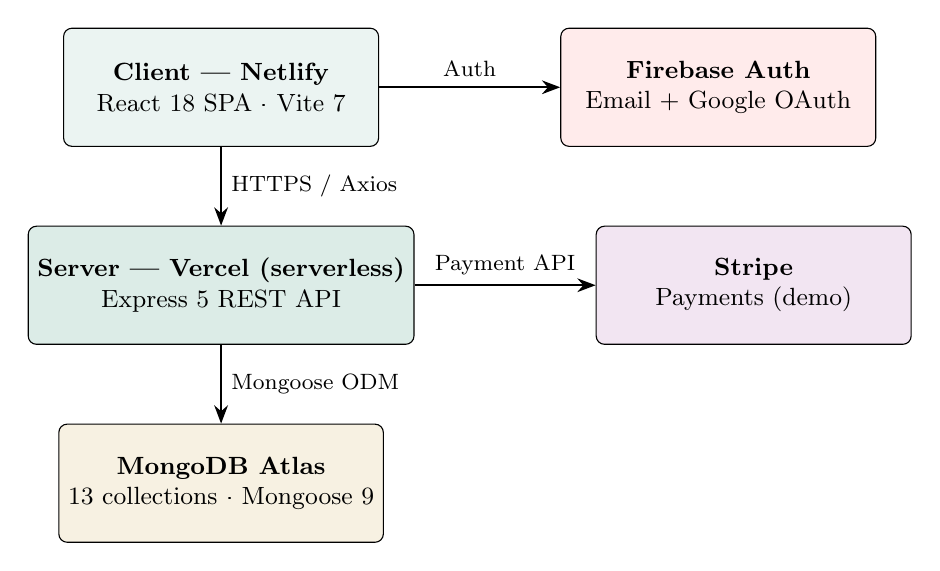
\begin{tikzpicture}[
  node distance=1.1cm,
  box/.style={draw, rounded corners=3pt, align=center, minimum width=4cm,
              minimum height=1.5cm, font=\small},
  arrow/.style={-Stealth, thick, font=\footnotesize}
]
\node[box, fill=emerald!8] (client) {\textbf{Client --- Netlify}\\React 18 SPA \textperiodcentered{} Vite 7};
\node[box, fill=emerald!14, below=1.0cm of client] (server)
   {\textbf{Server --- Vercel (serverless)}\\Express 5 REST API};
\node[box, fill=gold!14, below=1.0cm of server] (db)
   {\textbf{MongoDB Atlas}\\13 collections \textperiodcentered{} Mongoose 9};
\node[box, fill=red!8, right=2.3cm of client] (fb)
   {\textbf{Firebase Auth}\\Email + Google OAuth};
\node[box, fill=violet!10, right=2.3cm of server] (stripe)
   {\textbf{Stripe}\\Payments (demo)};
\draw[arrow] (client) -- node[right,font=\footnotesize]{HTTPS / Axios} (server);
\draw[arrow] (server) -- node[right,font=\footnotesize]{Mongoose ODM} (db);
\draw[arrow] (client) -- node[above,font=\footnotesize]{Auth} (fb);
\draw[arrow] (server) -- node[above,font=\footnotesize]{Payment API} (stripe);
\end{tikzpicture}
\caption{High-level three-tier system architecture of Nikah.}
\label{fig:arch}
\end{figure}

\section{Use-Case Analysis}
Four actors interact with the system. Their principal use cases are summarised
in Table~\ref{tab:usecases}; the inheritance relationship is that a
\emph{premium user} inherits every capability of a \emph{registered user} and
adds premium privileges.

\begin{table}[H]
\centering
\caption{Use-case summary by actor.}
\label{tab:usecases}
\small
\begin{tabularx}{\textwidth}{l X}
\toprule
\textbf{Actor} & \textbf{Representative use cases} \\
\midrule
Guest    & Register; log in; browse the home page; view success stories; use the contact form. \\
\addlinespace
Registered user &
Create / edit / view own biodata; search with filters; view biodata details;
add or remove favourites; request contact information; send and receive
messages; read notifications; view compatibility matches; see who viewed their
profile; browse recently-viewed profiles; view an activity feed; report a
profile; compare biodatas; submit a success story; toggle theme and language. \\
\addlinespace
Premium user &
Everything a registered user can do, plus: view contact information without a
per-request payment; unlimited contact requests; highlighted profile. \\
\addlinespace
Administrator &
View the analytics dashboard; manage users (search, promote/demote, grant or
revoke premium); approve premium requests; approve contact requests; moderate
success stories; read contact-form messages; handle reported profiles. \\
\bottomrule
\end{tabularx}
\end{table}

\begin{figure}[H]
\centering
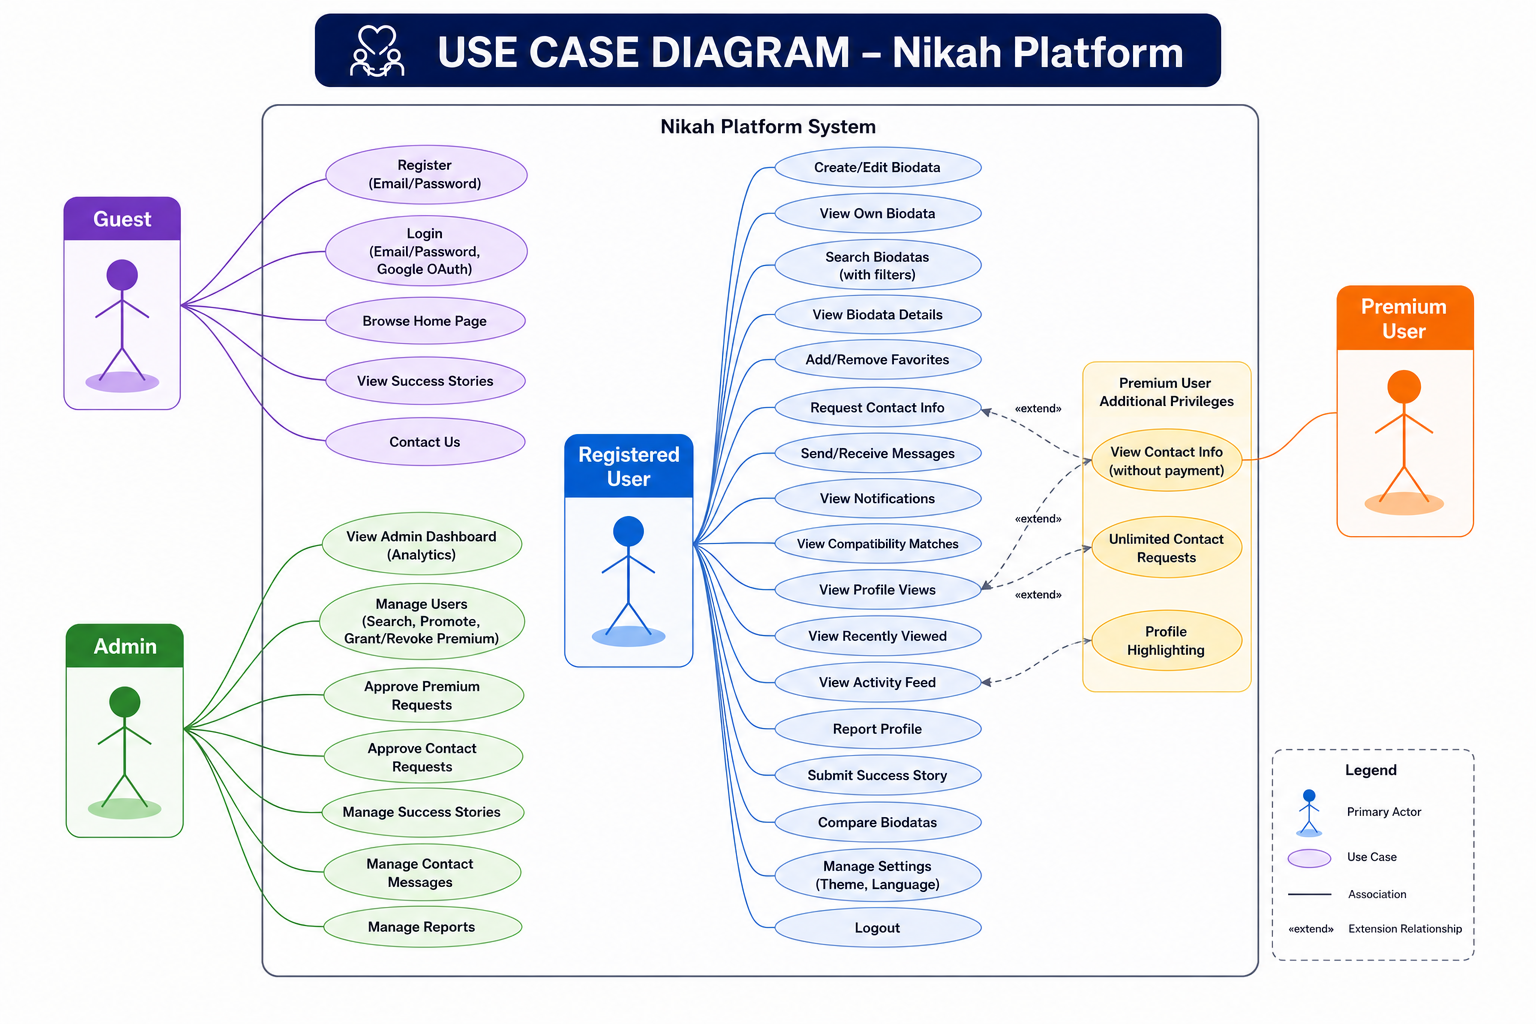
\includegraphics[width=\textwidth,keepaspectratio]{Image_and_Diagrams/SDP_Use_Case_Diagram.png}
\caption{System Use Case Diagram.}
\label{fig:usecase}
\end{figure}

\section{Context-Level Diagram (DFD-0)}
The context diagram (Figure~\ref{fig:dfd0}) shows the system as a single
process exchanging flows with its external entities: guests and members, the
Firebase authentication service, the MongoDB database and the Stripe payment
service.

\begin{figure}[H]
\centering
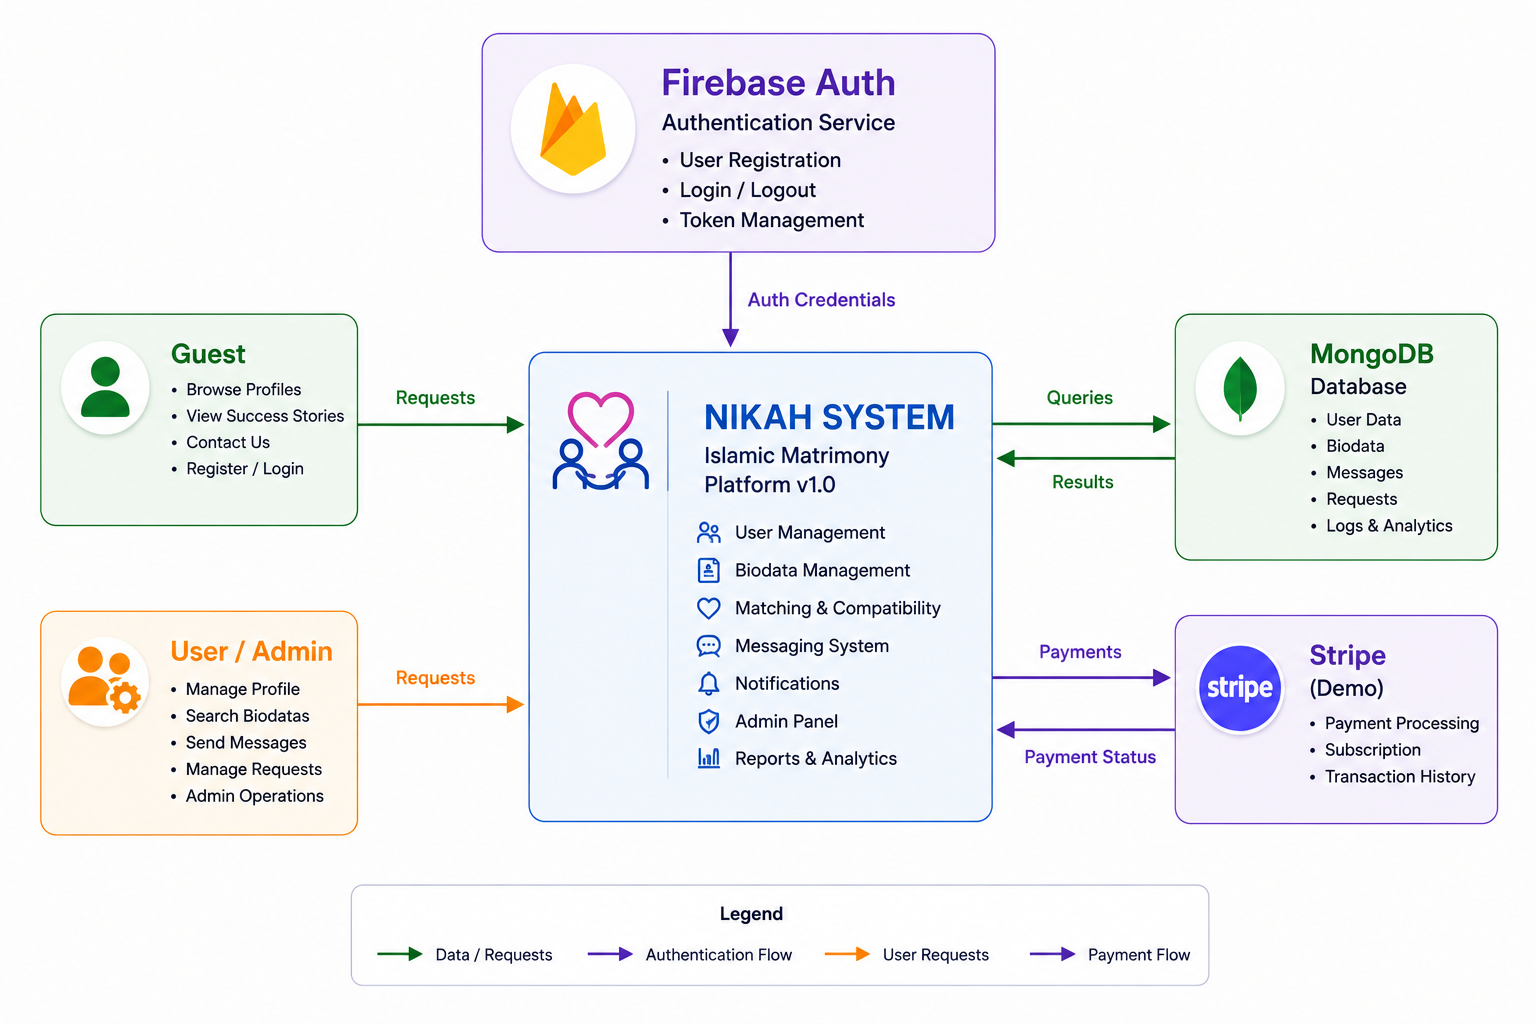
\includegraphics[width=\textwidth,keepaspectratio]{Image_and_Diagrams/Context_Level_Diagram_DFD_0.png}
\caption{Context-level diagram (DFD-0).}
\label{fig:dfd0}
\end{figure}

\section{Data-Flow Diagram (DFD-1)}
The first-level decomposition (Figure~\ref{fig:dfd1}) breaks the system into
six cooperating subsystems --- authentication, biodata management, contact
requests, payment, messaging and notifications --- all of which read from and
write to the shared MongoDB database.

\begin{figure}[H]
\centering
\safegfx{width=\textwidth,keepaspectratio}{dfd1.png}
\caption{First-level data-flow diagram (DFD-1).}
\label{fig:dfd1}
\end{figure}

\section{Database Schema}
The entity relationships among the thirteen collections are shown in
Figure~\ref{fig:erdiagram}. Indexes were added on frequently queried fields ---
\texttt{email}, \texttt{biodataId}, \texttt{biodataType},
\texttt{permanentDivision} and \texttt{age} --- to keep query latency low as
the data grows. Selected field-level detail is given in Table~\ref{tab:schema}.

\begin{figure}[H]
\centering
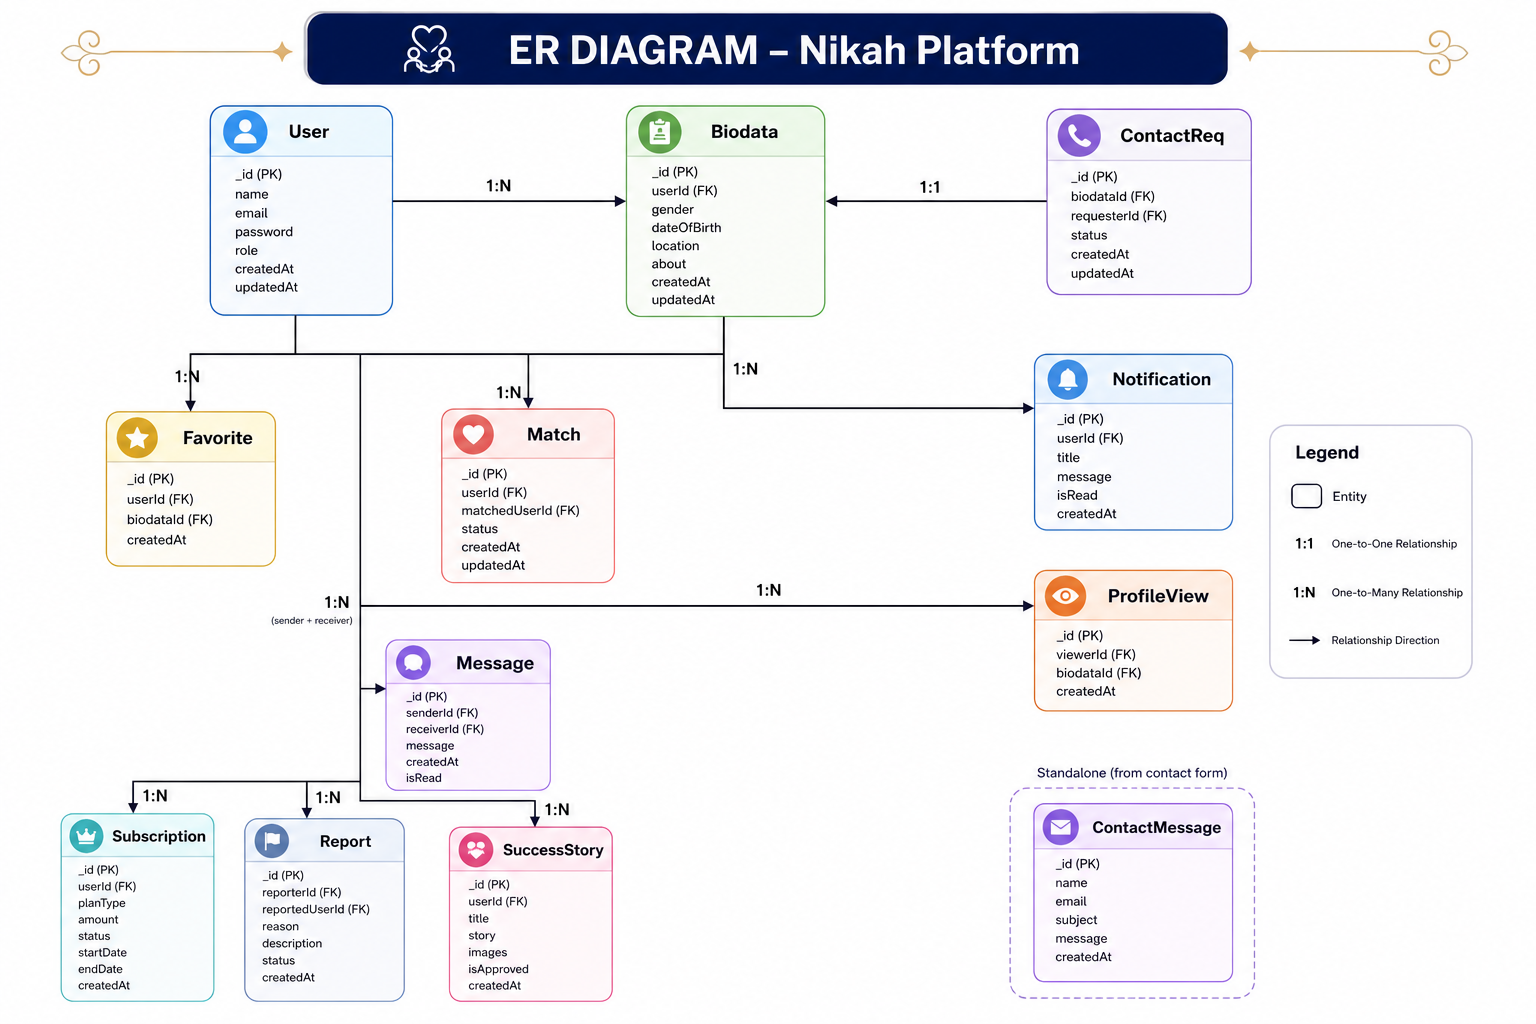
\includegraphics[width=\textwidth,keepaspectratio]{Image_and_Diagrams/SDP_ER_DIAGRAM.png}
\caption{Entity-relationship overview of the Nikah database.}
\label{fig:erdiagram}
\end{figure}

\begin{table}[H]
\centering
\caption{Selected schema field detail.}
\label{tab:schema}
\small
\begin{tabularx}{\textwidth}{l l X}
\toprule
\textbf{Model} & \textbf{Key field} & \textbf{Notes} \\
\midrule
User          & role                 & enum \texttt{['user','admin']}; \texttt{isPremium} boolean; \texttt{premiumRequestStatus} enum \\
Biodata       & biodataId            & unique auto-incrementing number; \texttt{biodataType} Male/Female; 7 divisions; occupation \& race enums \\
ContactRequest& status               & enum \texttt{['pending','approved']}; \texttt{paymentId} required \\
Match         & compatibilityScore   & numeric 0--100; \texttt{matchDetails} booleans; status enum \\
Message       & content              & \texttt{senderId}/\texttt{receiverId}; \texttt{isRead} flag; indexed by email \\
Notification  & type                 & six types (contact\_request, contact\_approved, premium\_approved, new\_message, profile\_viewed, system) \\
Report        & reason               & five reasons; status \texttt{pending/reviewed/resolved/dismissed} \\
Subscription  & plan                 & \texttt{basic/premium/gold}; payment method incl.\ bKash/Nagad/Rocket; status lifecycle \\
SuccessStory  & marriageDate         & 1--5 star rating; \texttt{pre('save')} hook auto-fills male/female biodata IDs \\
\bottomrule
\end{tabularx}
\end{table}

\section{Sequence Diagram}
The sequence diagram (Figure~\ref{fig:seqdiagram}) illustrates the execution flow for payment processing and contact request handling.

\begin{figure}[H]
\centering
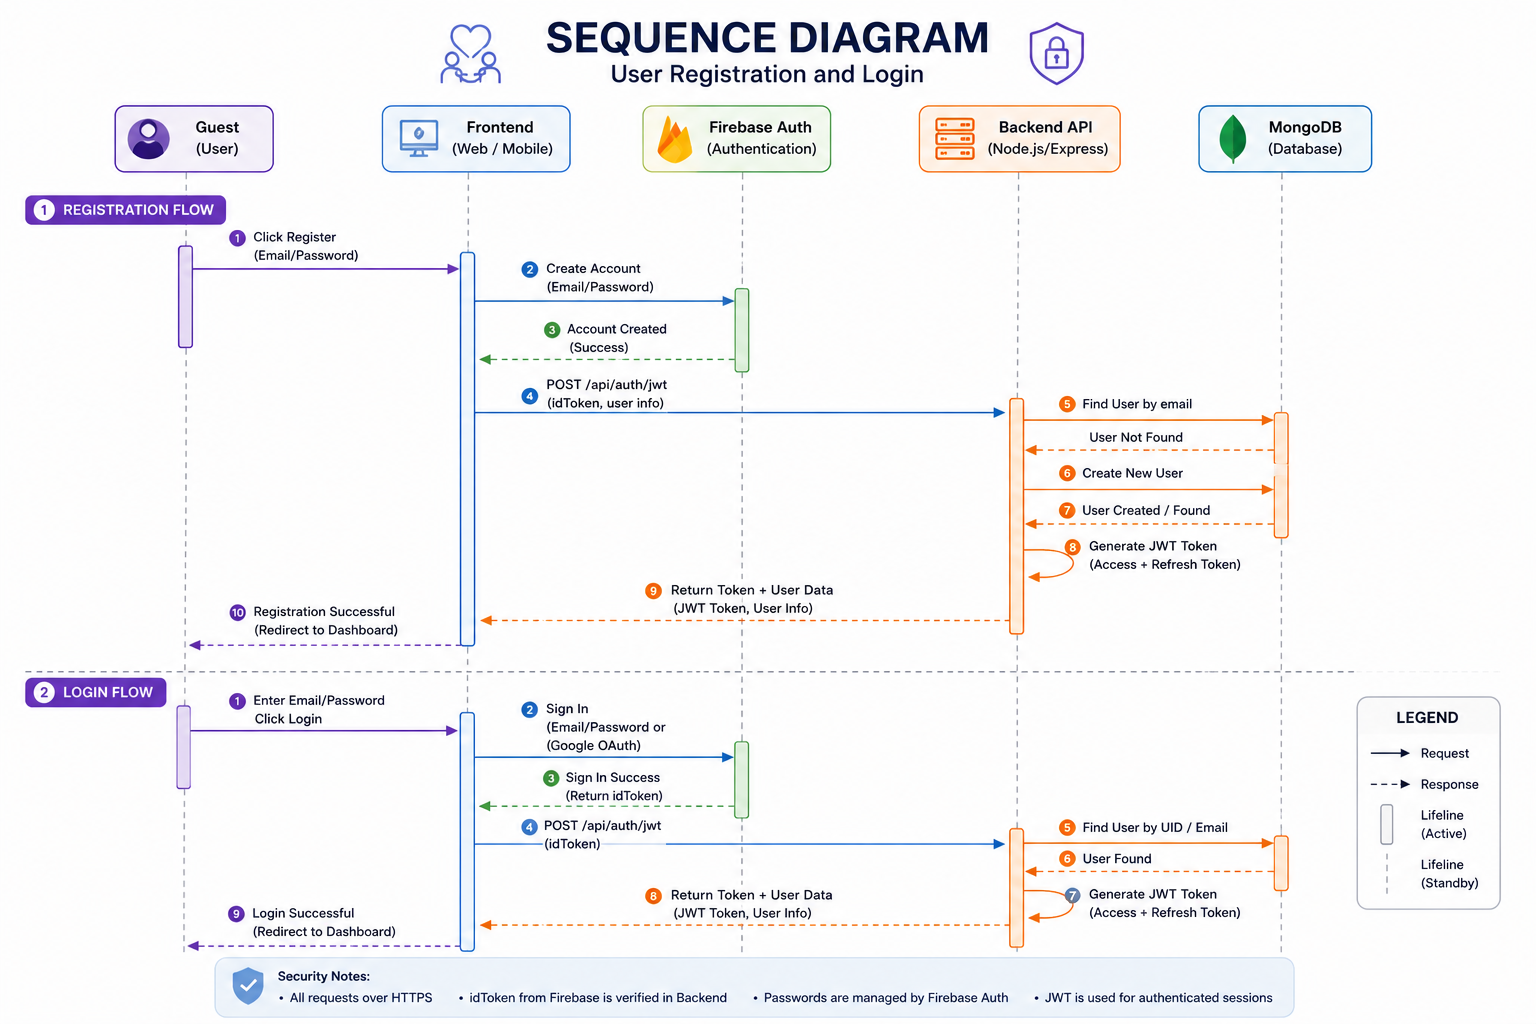
\includegraphics[width=\textwidth,keepaspectratio]{Image_and_Diagrams/SDP_Sequence_Diagram.png}
\caption{Sequence Diagram for Payment and Contact Requests.}
\label{fig:seqdiagram}
\end{figure}

\section{Activity Diagram}
The activity diagram (Figure~\ref{fig:actdiagram}) details the step-by-step user onboarding and matching workflow.

\begin{figure}[H]
\centering
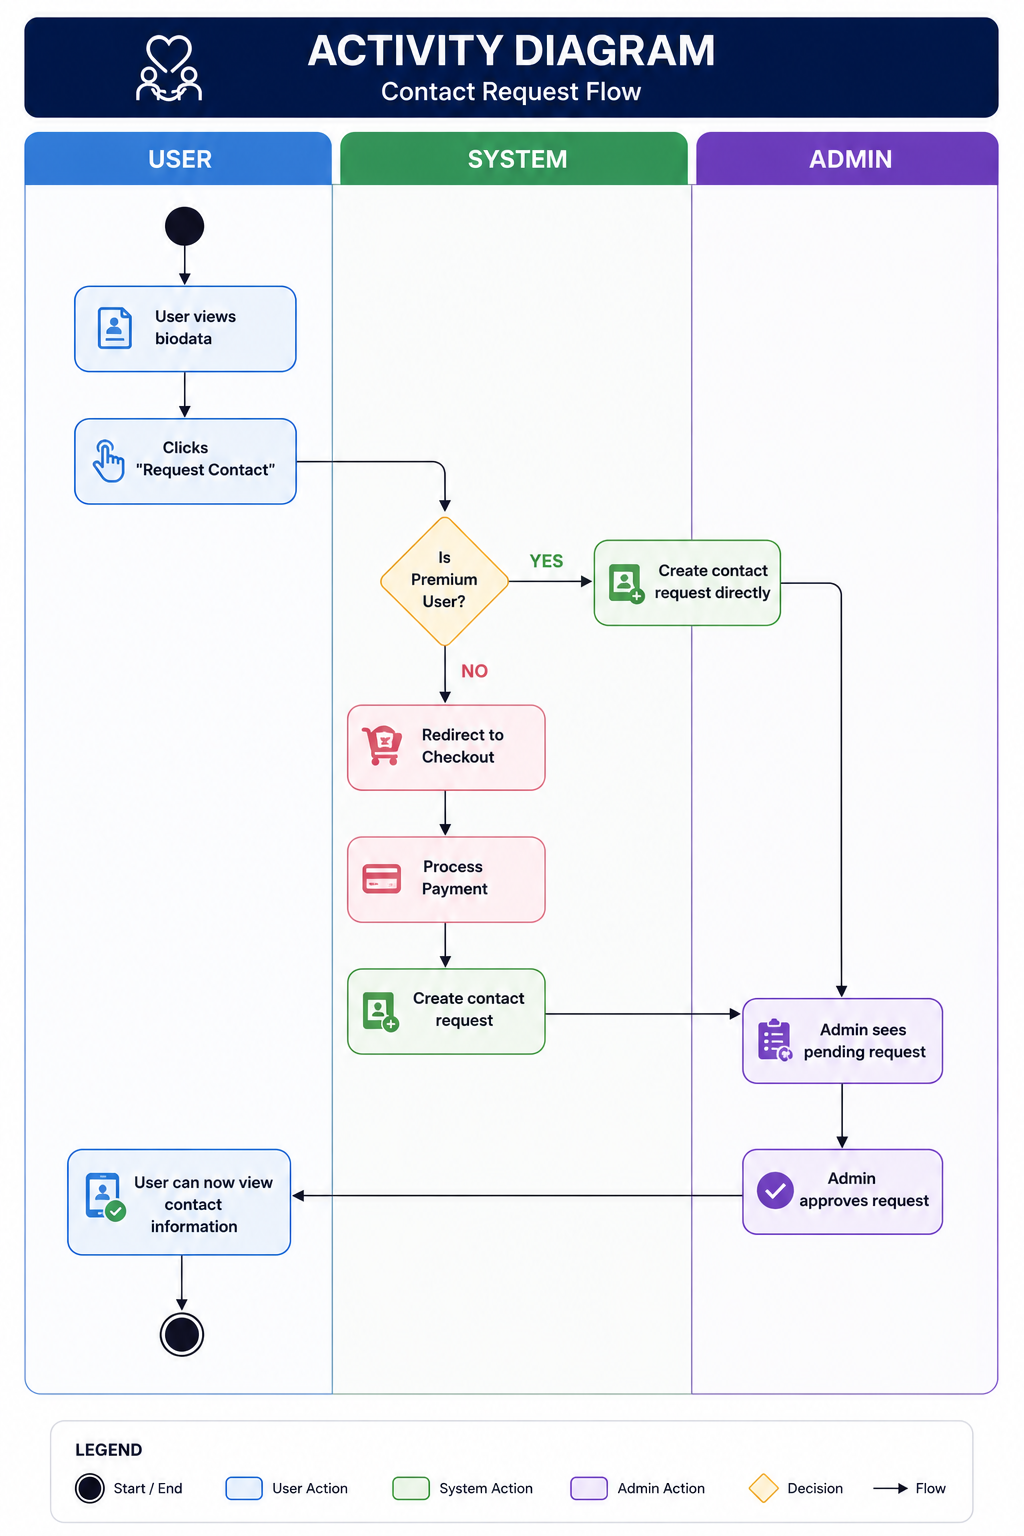
\includegraphics[width=\textwidth,keepaspectratio]{Image_and_Diagrams/SDP_Activity_Diagram.png}
\caption{Activity Diagram for user onboarding and matching.}
\label{fig:actdiagram}
\end{figure}

\section{Algorithms and Flowcharts}

\subsection{Compatibility Matching}
The matching algorithm compares a member's stored partner preferences against
every opposite-gender candidate and produces a weighted percentage score in the
range 0--100. Five criteria are evaluated, each contributing a fixed weight:
\textbf{deen (35\%)}, age range (25\%), height (15\%), division (15\%) and
occupation (10\%). Religion (\emph{deen}) is deliberately the single largest
factor, implementing the Prophetic guidance to prioritise religious commitment
when choosing a spouse (Sahih al-Bukhari~5090).

The deen sub-score itself combines four signals --- sect/madhhab (weight
$0.4$), prayer frequency ($0.25$), religious commitment ($0.25$) and religious
education ($0.10$) --- normalised by the signals actually present on both
profiles. A binary \texttt{deenMatch} flag is set when this normalised sub-score
reaches $0.70$. The secular factors contribute their full weight on an exact
match. Factors whose data is absent on either profile are excluded and the
final score is normalised by the sum of the weights actually computable, so
that profiles with sparse data are not unfairly penalised. Up to fifty
candidates are scored and the top twenty are returned, sorted in descending
order, each with a per-factor breakdown so members can see exactly what
matched. The simplified flowchart is shown in Figure~\ref{fig:matchflow}, and
the implementation in Figure~\ref{fig:compatibility}.

\begin{figure}[H]
\centering
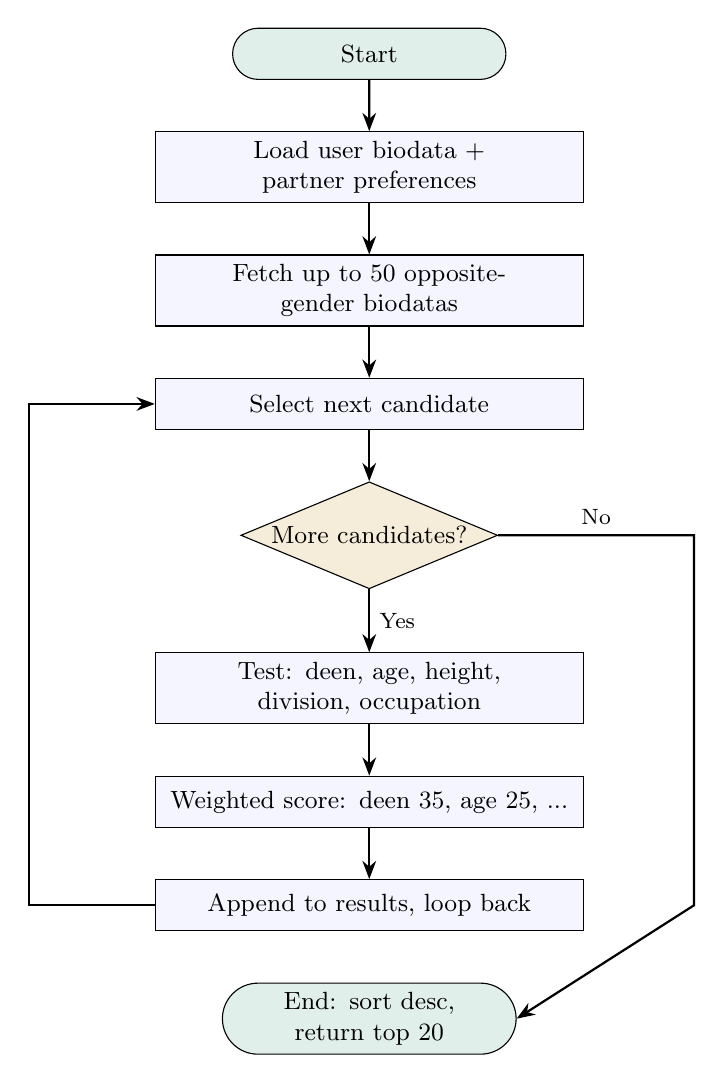
\begin{tikzpicture}[node distance=0.65cm and 0.9cm,
  startend/.style={draw, rounded rectangle, fill=emerald!12, align=center,
                   minimum height=0.65cm, text width=3.2cm, font=\small},
  proc/.style={draw, align=center, fill=blue!4, minimum height=0.65cm,
               text width=5.2cm, font=\small},
  dec/.style={draw, diamond, fill=gold!18, align=center, aspect=2.4,
              inner sep=1pt, font=\small},
  arr/.style={-Stealth, thick, font=\footnotesize}
]
\node[startend] (s) {Start};
\node[proc, below=of s] (p1) {Load user biodata + partner preferences};
\node[proc, below=of p1] (p2) {Fetch up to 50 opposite-gender biodatas};
\node[proc, below=of p2] (p3) {Select next candidate};
\node[dec, below=of p3] (d) {More candidates?};
\node[proc, below=of d, yshift=-0.15cm] (p4) {Test: deen, age, height, division, occupation};
\node[proc, below=of p4] (p5) {Weighted score: deen 35, age 25, ...};
\node[proc, below=of p5] (p6) {Append to results, loop back};
\node[startend, below=of p6] (e) {End: sort desc, return top 20};
\draw[arr] (s)--(p1); \draw[arr] (p1)--(p2); \draw[arr] (p2)--(p3);
\draw[arr] (p3)--(d);
\draw[arr] (d) -| node[above,pos=0.25]{No} ($(p6.east)+(1.4,0)$) -- (e.east);
\draw[arr] (d)-- node[right]{Yes} (p4);
\draw[arr] (p4)--(p5); \draw[arr] (p5)--(p6);
\draw[arr] (p6.west) -- ++(-1.6,0) |- (p3.west);
\end{tikzpicture}
\caption{Compatibility matching algorithm flowchart.}
\label{fig:matchflow}
\end{figure}

\begin{figure}[H]
\centering
\safegfx{width=\textwidth,keepaspectratio}{compatibility.png}
\caption{Compatibility scoring logic.}
\label{fig:compatibility}
\end{figure}

\subsection{Authentication Flow}
Two authentication paths exist. \textbf{Members} authenticate through Firebase
(email/password or Google) and the verified identity is exchanged for a
server JWT at \texttt{POST /api/auth/jwt}. \textbf{Administrators} authenticate
directly against environment-configured credentials at
\texttt{POST /api/auth/admin-login}, entirely outside Firebase. The flow is shown in Figure~\ref{fig:authflow}.

\begin{figure}[H]
\centering
\safegfx{width=\textwidth,keepaspectratio}{auth_flow.png}
\caption{Authentication flow (member and administrator paths).}
\label{fig:authflow}
\end{figure}

\subsection{Contact-Request Workflow}
\begin{figure}[H]
\centering
\safegfx{width=\textwidth,keepaspectratio}{contact_flow.png}
\caption{Contact-information request workflow.}
\label{fig:contactflow}
\end{figure}

%==============================================================================
\chapter{Implementation}
%==============================================================================

\section{Front-End / Interface Design}
The front end is a React~18 single-page application built with Vite~7. It is
organized into \textbf{pages} (route-level components), \textbf{layouts} (shared
\texttt{MainLayout} with navbar/footer and \texttt{DashboardLayout} with
sidebar), and \textbf{reusable components}, including twenty-four
shadcn/ui primitives under \texttt{components/ui}.

\paragraph{Design system.} The UI is built on \textbf{shadcn/ui} (new-york
style, JSX, slate base) atop \textbf{Radix UI} primitives and styled with
\textbf{Tailwind CSS} in \texttt{darkMode:'class'} mode. The brand tokens are a
custom \textbf{emerald-and-gold} palette --- \texttt{-{}-primary} deep emerald
(HSL \texttt{160 84\% 24\%}) with a champagne-gold accent --- exposed as CSS
custom properties and consumed through Tailwind. The \texttt{Inter} and
\texttt{Outfit} typefaces carry Latin text and \texttt{Noto Sans Bengali}
carries Bangla. Custom utilities (\texttt{gradient-islamic},
\texttt{gradient-gold}, \texttt{glass-nav}) and animations
(\texttt{fade-in-up}, \texttt{shimmer}, \texttt{marquee}) reinforce the brand.

\paragraph{Routing.} React Router~7 with \texttt{createBrowserRouter} defines
thirty-four routes: twelve public routes under \texttt{MainLayout}, fourteen
protected user-dashboard routes, seven administrator routes, and a catch-all
\texttt{NotFound}. Guard components \texttt{PrivateRoute} and
\texttt{AdminRoute} gate access based on authentication and role.

\paragraph{State management.} Three React contexts manage global state:
\textbf{AuthContext} (Firebase user or synthetic admin user, JWT, role, premium
status, loading), \textbf{ThemeContext} (dark/light with
\texttt{localStorage} persistence and system-preference fallback), and
\textbf{LanguageContext} (English/Bangla with dot-path translation lookup over
707-line dictionaries). Provider nesting is
\texttt{HelmetProvider $\to$ LanguageProvider $\to$ ThemeProvider $\to$
QueryClientProvider $\to$ AuthProvider}.

\paragraph{Server state.} TanStack React Query manages all API data with a
five-minute stale time, a single retry, and refetch-on-window-focus disabled.

\paragraph{API layer.} A single Axios instance reads its base URL from
\texttt{VITE\_API\_URL}. A request interceptor attaches the JWT from
\texttt{localStorage} as a Bearer token and the active locale as an
\texttt{Accept-Language} header; a response interceptor detects HTTP~401,
clears the token, and dispatches an \texttt{'unauthorized'} window event that
\texttt{AuthContext} listens for in order to log the user out globally.

\paragraph{UI libraries.} Framer Motion for transitions, React Helmet Async for
SEO, React Hot Toast and SweetAlert2 for feedback, and Recharts for the
administrator charts.

\section{Back-End}
The back end is an Express~5 application (CommonJS). The entry point configures
CORS with an origin allow-list (the configured client URL, localhost, any
\texttt{*.netlify.app} and \texttt{*.vercel.app} origin, and origin-less
requests such as mobile clients), enables JSON and cookie parsing, mounts
seventeen routers under \texttt{/api/}, and registers a 404 handler and a
centralized error handler. All business logic is implemented inline within the
route handlers.

\paragraph{Middleware.} Three functions control access:
\texttt{verifyToken} extracts and verifies the JWT, lazily provisions a
\texttt{User} document if the decoded email is new, and refreshes
\texttt{req.user} with the current role and premium status;
\texttt{verifyAdmin} treats the environment-configured \texttt{ADMIN\_EMAIL}
as the single source of truth for administrator identity and actively
\emph{downgrades} any database user whose email does not match but who holds
\texttt{role:'admin'}; and \texttt{verifyPremium} rejects non-premium callers
with HTTP~403.

\paragraph{Environment-based administrator login.}
This is a deliberate security design. The administrator does \emph{not} use
Firebase. At \texttt{POST /api/auth/admin-login} (Figure~\ref{fig:adminlogin})
the server compares the supplied credentials against
\texttt{ADMIN\_EMAIL} and \texttt{ADMIN\_PASSWORD}. The password is accepted
either as a \texttt{bcrypt} hash \emph{or} as plain text (dual-mode compare),
the email comparison is case-insensitive, and on success the server upserts a
\texttt{User} with \texttt{role:'admin'} and \texttt{isPremium:true} and issues
a seven-day JWT carrying a custom \texttt{adminLogin:true} claim. Because the
client sets \texttt{isAdmin} directly from this response, the administrator can
enter \texttt{/dashboard/admin/*} without ever touching Firebase.

\begin{figure}[H]
\centering
\safegfx{width=\textwidth,keepaspectratio}{admin_login_flow.png}
\caption{Environment-based administrator login (server, simplified).}
\label{fig:adminlogin}
\end{figure}

\paragraph{Route modules.} The seventeen routers expose seventy handlers across
authentication, biodata, contact requests, contact messages, favourites,
matches, messages, notifications, payments, profile views, recently-viewed
records, reports, statistics, subscriptions, success stories, analytics and
administration. Selected endpoints are listed in Appendix~\ref{app:endpoints}.

\paragraph{Database models.} Thirteen Mongoose schemas (Table~\ref{tab:collections})
carry field validation (required fields, enums, min/max values), timestamps,
and indexes on hot fields. The \texttt{Biodata} model uses a unique
auto-incrementing \texttt{biodataId}, and the \texttt{SuccessStory} model uses
a \texttt{pre('save')} hook to auto-classify the male/female biodata IDs.

\paragraph{Security.} JWTs expire after seven days; administrator identity is
pinned to a single environment variable and stale administrator roles are
actively demoted; contact information is hidden from non-premium users who do
not own the biodata; CORS validates origins; and all secrets live in
environment variables. The \texttt{.env} file is git-ignored.

\section{Modules and Features}
The following functional modules were implemented (fifteen core modules, with five additional Islamic-specific modules marked with $\star$):

\begin{enumerate}
  \item \textbf{Authentication} --- Firebase email/password and Google for
        members, plus a separate secure, environment-based administrator login.
  \item \textbf{Biodata management} --- create and update biodata with sixteen
        or more fields, auto-incrementing IDs and automatic age calculation
        from date of birth, including a Deen \& Islamic profile section
        (sect, prayer, modesty, religious commitment, mahr preference, lifestyle).
        $\star$
  \item \textbf{Search and discovery} --- filter by gender, division, age range
        and occupation, with pagination (twenty per page) and sort options.
  \item \textbf{Contact-request system} --- request contact info with a Stripe
        payment for non-premium members, an administrator approval workflow,
        and a premium bypass; requests to wali-protected profiles are routed
        through guardian approval. $\star$
  \item \textbf{Favourites} --- add and remove bookmarks with duplicate
        prevention.
  \item \textbf{Messaging} --- inbox, sent and conversation threading with
        unread tracking and notification generation, plus halal initial-contact
        templates and an optional CC-the-wali feature. $\star$
  \item \textbf{Notifications} --- notification types (including wali-related)
        with unread badge, mark-as-read, mark-all-read and delete.
  \item \textbf{Compatibility matching} --- 0--100 weighted scoring across five
        criteria (deen, age, height, division, occupation) with religion as the
        dominant factor and a per-factor breakdown and mutual-score view.
        $\star$
  \item \textbf{Profile-view tracking} --- records views with self-view and
        one-hour duplicate suppression, and reports total and unique viewers.
  \item \textbf{Recently viewed} --- a per-user history of recently browsed
        biodata, kept in sync between \texttt{localStorage} and the server and
        automatically trimmed to twenty entries.
  \item \textbf{Premium subscription} --- three plans (Basic free, Premium, and
        Gold) with Stripe payment, contact-info access and profile highlighting.
  \item \textbf{Reporting} --- report profiles for five reasons, with an
        administrator review and resolve/dismiss workflow.
  \item \textbf{Success stories} --- married members submit a story with partner
        ID, couple photo, marriage date, rating and text, moderated by an
        administrator.
  \item \textbf{Administration dashboard} --- analytics charts for user growth,
        gender, location and age distribution, plus user management, premium and
        contact approvals, verification approvals, content moderation and revenue.
  \item \textbf{Wali (guardian) oversight} $\star$ --- members enable wali
        oversight and supply guardian details; each contact request to a
        protected profile generates a single-use approval link the wali uses to
        approve or decline before contact details are shared.
  \item \textbf{Profile verification} $\star$ --- members request
        verification via NID, imam endorsement or a community-leader reference;
        administrators review and grant a verified badge that signals trust.
  \item \textbf{Islamic guidance hub} $\star$ --- bilingual, referenced
        articles on marriage in Islam, choosing a spouse, istikhara, mahr, wali
        and witnesses, and marital rights, plus an ``Ask an Imam'' route.
  \item \textbf{Internationalization and theming} --- English/Bangla switching
        persisted to storage and sent as a request header, plus a class-based
        dark/light theme with a system-preference fallback.
\end{enumerate}

%==============================================================================
\chapter{User Manual}
%==============================================================================

\section{System Requirements}

\subsection{Hardware Requirements}
\begin{table}[H]
\centering
\caption{Hardware requirements.}
\label{tab:hw}
\small
\begin{tabularx}{\textwidth}{l X X}
\toprule
\textbf{Component} & \textbf{Minimum} & \textbf{Recommended} \\
\midrule
Processor & Intel Core i3 / AMD Ryzen 3 & Intel Core i5 / AMD Ryzen 5 \\
RAM       & 4 GB                        & 8 GB \\
Storage   & 1 GB free                   & 5 GB free \\
Display   & 1366$\times$768             & 1920$\times$1080 \\
Internet  & 2 Mbps                      & 10 Mbps \\
Device    & Desktop, laptop, tablet, phone & Any modern-browser device \\
\bottomrule
\end{tabularx}
\end{table}

\subsection{Software Requirements}
\paragraph{For users.} Windows~10+, macOS~11+, Linux, Android~10+ or iOS~14+;
Chrome~90+, Firefox~90+, Safari~14+ or Edge~90+; JavaScript enabled; an
internet connection.
\paragraph{For local development.} Windows~10+, macOS~11+ or Ubuntu~20.04+;
Node.js v18+ (v24.10.0 recommended); npm v9+; a MongoDB Atlas account (free
tier) or MongoDB v6.0+ locally; VS Code; Git v2.30+; and a Firebase Console
project with Authentication enabled.

\section{User Interfaces}

\subsection{Panel A --- Public Pages}
The home page presents a hero with calls to action (``Get Started'' and
``Browse Biodatas''), featured premium profiles, an animated statistics
counter, a ``How It Works'' section and a success-story gallery with ratings,
all wrapped by a glass-style navbar and a footer with a newsletter form. The
\textbf{biodatas listing} page offers a filter sidebar (biodata type, division,
age range, occupation) over a paginated grid of cards; the \textbf{biodata
details} page exposes contact-request, favourite and report actions; the
\textbf{login} and \textbf{register} pages offer Firebase email/password and
Google; the dedicated \textbf{admin login} page is a separate, server-side
credential form. Static pages cover About, Contact (with a form), Privacy and
Terms, and a success-stories gallery and a biodata comparison page are also
available. Representative interfaces are illustrated in
Figures~\ref{fig:home}--\ref{fig:listing}.

\uifig{Home page hero with branding and primary calls to action.}{fig:home}{fig5_1_home.png}
\uifig{Biodata details page with contact-request and favourite actions.}{fig:details}{fig5_2_details.png}
\uifig{Biodatas listing with filter sidebar and paginated card grid.}{fig:listing}{fig5_3_listing.png}

\subsection{Panel B --- User Dashboard}
The dashboard provides an overview (biodata status, unread messages,
favourites, profile views, activity feed and quick actions); \textbf{edit /
view biodata} (with auto-calculated age and all seven divisions); \textbf{edit
biodata} (full form with sixteen or more fields); \textbf{messages} (inbox,
sent, conversation); \textbf{notifications}; \textbf{matches} (cards with 0--100
scores and breakdowns); \textbf{favourites}; \textbf{contact requests};
\textbf{profile views}; \textbf{recently viewed}; \textbf{settings} (theme,
language, account); and \textbf{Got Married} (success-story submission).

\uifig{User dashboard overview with summary cards and activity feed.}{fig:userdash}{fig5_4_userdash.png}
\uifig{Compatibility matches with percentage scores and breakdowns.}{fig:matches}{fig5_5_matches.png}

\subsection{Panel C --- Admin Panel}
The administrator dashboard shows stat cards, an area chart for thirty-day user
growth, a pie chart for gender distribution, a bar chart for location
statistics, an age-distribution chart, and a recent-activity table. Further
tabs cover \textbf{manage users} (search, promote/demote, grant or revoke
premium), \textbf{approved premium}, \textbf{approved contacts},
\textbf{contact messages}, \textbf{success stories} moderation, and
\textbf{reported profiles}.

\uifig{Administrator dashboard with analytics charts and stat cards.}{fig:admindash}{fig5_6_admindash.png}
\uifig{Manage users table with role and premium controls.}{fig:manageusers}{fig5_7_manageusers.png}

\subsection{Login Credentials}
\begin{description}[leftmargin=1.5em]
  \item[\textbf{Administrator Access:}]
        The administrator authenticates through the dedicated secret route \texttt{/admin-login} using the environment-configured credentials:
        \begin{itemize}
          \item \textbf{E-mail:} \texttt{ummati2025@gmail.com}
          \item \textbf{Password:} \texttt{nikahteamsdp04@}
        \end{itemize}
        Public user registration with the administrator e-mail address is strictly restricted by system security policies.
  \item[\textbf{Test Member Access:}]
        Regular members can register via \texttt{/register} or authenticate with test member credentials:
        \begin{itemize}
          \item \textbf{E-mail:} \texttt{user@test.com}
          \item \textbf{Password:} \texttt{User@123}
        \end{itemize}
\end{description}

\section{Getting Started}
Clone the repository, run \texttt{npm install} in both \texttt{client/} and
\texttt{server/}, copy \texttt{server/.env.example} to \texttt{server/.env}
and fill in \texttt{MONGODB\_URI}, \texttt{JWT\_SECRET}, \texttt{CLIENT\_URL},
\texttt{ADMIN\_EMAIL}, \texttt{ADMIN\_PASSWORD} and (optionally)
\texttt{STRIPE\_SECRET\_KEY}, then start the API (\texttt{npm run dev}) and the
client (\texttt{npm run dev}).

%==============================================================================
\chapter{Conclusion}
%==============================================================================

\section{Conclusion}
Nikah matured into a full-featured matrimony platform that addresses real gaps
in the market for Bangladeshi Muslims. The final system comprises thirteen
database collections, seventy API route handlers across seventeen modules, and
fifteen functional modules spanning authentication, biodata management, search,
messaging, matching, payments and administration. The front end is responsive,
bilingual and dark-mode capable, built on a shadcn/ui emerald-and-gold design
system, and administrators are equipped with a proper analytics dashboard.

Security was treated as a first-class concern. JWT authentication with
role-based access control, contact-information gating, a dedicated
environment-based administrator login that is isolated from Firebase, an
origin-validated CORS policy, and active demotion of stale administrator roles
combine to keep the platform locked down. The deployment is live --- the API on
Vercel, the front end on Netlify and the database on MongoDB Atlas, all on free
tiers. Just as importantly, the features were designed around Islamic values
and now back that claim with real functionality: deen-weighted compatibility
matching (with religion as the largest scoring factor), wali (guardian)
oversight of every contact request to a protected profile, NID/imam profile
verification, halal-communication message templates, mahr transparency, an
Islamic guidance hub, contact gating for privacy, and parent-name fields for
family involvement.

\section{Limitations}
\begin{enumerate}
  \item \textbf{No native mobile application.} The web version is responsive,
        but native iOS and Android apps with push notifications would improve
        reach.
  \item \textbf{Payments run in demonstration mode.} Stripe is wired up but
        does not process real transactions, and local gateways such as bKash,
        Nagad and Rocket are not integrated.
  \item \textbf{No real-time transport.} Messaging and notifications operate on
        a request-response cycle; WebSockets would make chat instantaneous.
  \item \textbf{Rule-based matching.} The engine is a transparent weighted model
        (deen, age, height, division, occupation); machine learning could
        produce more nuanced recommendations from interaction data.
  \item \textbf{Verification is manual.} Profiles can be marked verified through
        admin review of NID/imam references, but the flow is not yet wired to an
        automated identity provider.
  \item \textbf{Single administrator identity.} Administrator access is pinned
        to one environment-configured account; a permission hierarchy would be
        more flexible.
  \item \textbf{Two languages only.} English and Bangla are covered; Arabic and
        Urdu would broaden reach.
\end{enumerate}

\section{Future Works}
Priority directions for future work include native mobile applications (React
Native); AI-powered matchmaking that learns from interaction patterns;
WebRTC-based voice and video calling for premium members; automated background
verification (connecting the existing NID/imam verification flow to a real
identity provider for education and employment checks); additional languages;
real payment integration with Stripe, bKash, Nagad and Rocket; real-time wali
email delivery (currently stubbed, with a magic-link fallback); advanced
analytics and match-success prediction; wedding-planning tools (vendor
directories, checklists, budgets); deeper community features (live scholar
consultations); and real-time chat with typing indicators and read receipts.

%==============================================================================
%  BACK MATTER
%==============================================================================
%---------- References ----------
\begin{thebibliography}{99}
\addcontentsline{toc}{chapter}{References}

\bibitem{react}      React. ``React Documentation.'' \url{https://react.dev/}, 2026.
\bibitem{vite}       Vite. ``Vite --- Next Generation Frontend Tooling.'' \url{https://vite.dev/}, 2026.
\bibitem{router}     React Router. ``React Router Documentation.'' \url{https://reactrouter.com/}, 2026.
\bibitem{tailwind}   Tailwind Labs. ``Tailwind CSS Documentation.'' \url{https://tailwindcss.com/docs}, 2026.
\bibitem{shadcn}     shadcn. ``shadcn/ui --- Build Your Component Library.'' \url{https://ui.shadcn.com/}, 2026.
\bibitem{radix}      Radix UI. ``Radix Primitives.'' \url{https://www.radix-ui.com/}, 2026.
\bibitem{query}      TanStack. ``TanStack Query Documentation.'' \url{https://tanstack.com/query/}, 2026.
\bibitem{node}       OpenJS Foundation. ``Node.js.'' \url{https://nodejs.org/}, 2026.
\bibitem{express}    OpenJS Foundation. ``Express --- Fast, unopinionated, minimalist web framework for Node.js.'' \url{https://expressjs.com/}, 2026.
\bibitem{mongo}      MongoDB, Inc. ``MongoDB Documentation.'' \url{https://www.mongodb.com/docs/}, 2026.
\bibitem{mongoose}   Mongoose. ``Mongoose ODM Documentation.'' \url{https://mongoosejs.com/docs/}, 2026.
\bibitem{firebase}   Google. ``Firebase Authentication.'' \url{https://firebase.google.com/docs/auth}, 2026.
\bibitem{jwt}        IETF. ``JSON Web Tokens.'' \url{https://jwt.io/}, 2026.
\bibitem{stripe}     Stripe. ``Stripe API Documentation.'' \url{https://stripe.com/docs/api}, 2026.
\bibitem{axios}      Axios. ``Axios HTTP Client.'' \url{https://axios-http.com/}, 2026.
\bibitem{framer}     Framer. ``Framer Motion.'' \url{https://www.framer.com/motion/}, 2026.
\bibitem{recharts}   Recharts. ``Recharts --- composable charting library.'' \url{https://recharts.org/}, 2026.
\bibitem{atlas}      MongoDB, Inc. ``MongoDB Atlas Documentation.'' \url{https://www.mongodb.com/docs/atlas/}, 2026.
\bibitem{vercel}     Vercel. ``Vercel Deployment Documentation.'' \url{https://vercel.com/docs}, 2026.
\bibitem{netlify}    Netlify. ``Netlify Documentation.'' \url{https://docs.netlify.com/}, 2026.
\bibitem{bcrypt}     dcodeIO. ``bcrypt.js.'' \url{https://github.com/dcodeIO/bcrypt.js}, 2026.
\bibitem{wcag}       W3C. ``Web Content Accessibility Guidelines (WCAG) 2.1.'' \url{https://www.w3.org/WAI/WCAG21/quickref/}, 2026.
\bibitem{bukhari}    Sunnah.com. ``Sahih al-Bukhari --- Book of Marriage.'' \url{https://sunnah.com/bukhari}, 2026.
\bibitem{bayhaqi}    al-Bayhaqi. \emph{Hadith on marriage fulfilling half of one's faith.}
\bibitem{lucide}     Lucide. ``Lucide Icons.'' \url{https://lucide.dev/}, 2026.
\bibitem{sweetalert} SweetAlert2. ``A beautiful, responsive, customizable replacement for JavaScript's popup boxes.'' \url{https://sweetalert2.github.io/}, 2026.
\bibitem{noto}       Google. ``Noto Sans Bengali.'' \url{https://fonts.google.com/noto}, 2026.
\bibitem{dfd}        Lucidchart. ``What is a Data Flow Diagram.'' \url{https://www.lucidchart.com/pages/data-flow-diagram}, 2026.
\bibitem{usecase}    Creately. ``Use Case Diagram Tutorial.'' \url{https://creately.com/guides/use-case-diagram-tutorial/}, 2026.
\bibitem{arch}       InterviewBit. ``System Architecture Tutorial.'' \url{https://www.interviewbit.com/blog/system-architecture/}, 2026.

\end{thebibliography}

%==============================================================================
%  APPENDICES
%==============================================================================
\appendix

\chapter{Glossary and Supplementary Material}
\label{app:glossary}

\section{Glossary of Terms}
\begin{table}[H]
\centering
\small
\begin{tabularx}{\textwidth}{l X}
\toprule
\textbf{Term} & \textbf{Meaning} \\
\midrule
Nikah         & The Islamic marriage contract. \\
Biodata       & A matrimonial profile with personal, family and preference details. \\
JWT           & JSON Web Token --- a compact token format for authentication. \\
RBAC          & Role-Based Access Control. \\
REST API      & A web API that follows REST conventions. \\
MERN          & MongoDB, Express, React and Node.js. \\
ODM           & Object Document Mapping between code objects and database documents. \\
i18n          & Internationalization. \\
CORS          & Cross-Origin Resource Sharing --- a browser security mechanism. \\
Stripe        & Online payment-processing platform. \\
Firebase      & Google's application platform (used here for authentication). \\
Vercel        & Cloud platform for serverless and static deployment. \\
Netlify       & Cloud platform for front-end deployment. \\
WCAG          & Web Content Accessibility Guidelines. \\
DFD           & Data Flow Diagram. \\
ER Diagram    & Entity-Relationship Diagram. \\
Hijab         & Islamic concept of modesty and privacy. \\
Wali          & Islamic marriage guardian whose consent is required for a valid nikah. \\
Halal         & Permissible under Islamic law. \\
Deen          & Religion / religious commitment (Arabic). \\
Mahr          & The mandatory bridal gift given by the husband to the wife at marriage (Qur'an 4:4). \\
Istikhara     & The prayer of seeking Allah's guidance before a decision. \\
Madhhab       & A school of Islamic jurisprudence (e.g. Hanafi, Shafi'i). \\
Sadaqah Jariyah & Perpetual charity --- continuous good deeds. \\
bKash/Nagad/Rocket & Mobile financial services in Bangladesh. \\
\bottomrule
\end{tabularx}
\end{table}

\section{Key API Endpoints}
\label{app:endpoints}
\begin{table}[H]
\centering
\small
\begin{tabularx}{\textwidth}{l l X l}
\toprule
\textbf{Method} & \textbf{Endpoint} & \textbf{Purpose} & \textbf{Auth} \\
\midrule
POST   & /api/auth/jwt                & Exchange Firebase identity for a server JWT & Public \\
POST   & /api/auth/admin-login        & Environment-based administrator login        & Public \\
GET    & /api/auth/me                 & Current user                                & Token \\
GET    & /api/biodata                 & List biodata with filters                   & Public \\
GET    & /api/biodata/:id             & Get one biodata                             & Mixed \\
POST   & /api/biodata                 & Create or update biodata                    & Token \\
POST   & /api/contact-requests        & Request contact information                 & Token \\
GET    & /api/matches                 & Compatibility matches                       & Token \\
GET    & /api/matches/with/:id        & Mutual compatibility with a biodata         & Token \\
GET    & /api/messages/inbox          & Received messages                           & Token \\
POST   & /api/messages                & Send a message                              & Token \\
GET    & /api/notifications           & Notifications                               & Token \\
POST   & /api/favorites               & Add a favourite                             & Token \\
GET    & /api/recently-viewed         & Recently viewed history                     & Token \\
POST   & /api/subscriptions           & Create a subscription                       & Token \\
POST   & /api/payment/create-payment-intent & Create a Stripe payment intent        & Token \\
GET    & /api/stats/public            & Public platform statistics                  & Public \\
GET    & /api/analytics/stats         & Administrator analytics                     & Admin \\
GET    & /api/admin/users             & List all users                              & Admin \\
PATCH  & /api/admin/users/:id/make-admin & Promote a user to administrator           & Admin \\
\bottomrule
\end{tabularx}
\end{table}

\section{Project Timeline}
\begin{figure}[H]
\centering
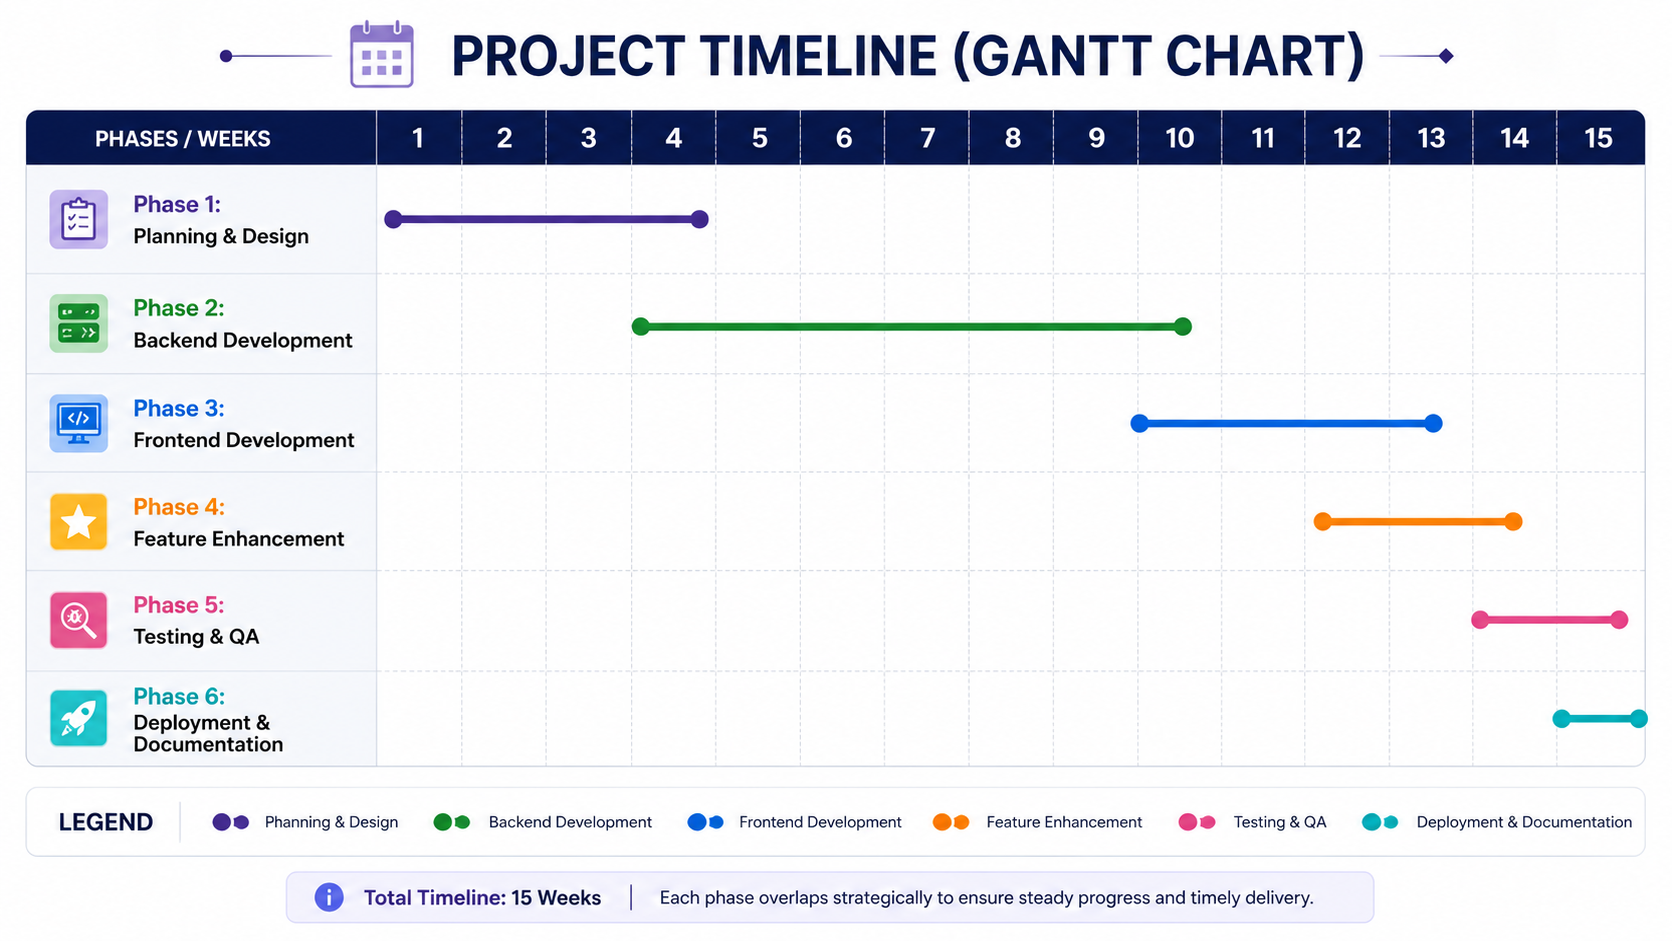
\includegraphics[width=\textwidth,keepaspectratio]{Image_and_Diagrams/SDP_Projecr_Timeline.png}
\caption{Project Timeline and Release Milestones.}
\label{fig:timeline}
\end{figure}

\vspace{1.5cm}
\begin{center}
\textit{--- End of Document ---}
\end{center}

\end{document}
